{
Hvad er et topografisk kort? Forklar. Eksempler på topografiske kort kan
ses i figur \ref{topography_plus} og \ref{topography_times}.

Vi vil nu beskrive en metode hvorved regioner bliver tildelt en
omkostning. Denne omkostning beregnes ud fra regionens placering i
billedet på baggrund af et topografisk kort. Således vil regioner ikke
blive vurderet efter hvorvidt de ligger i det gyldne snit eller ej, men
efter \emph{hvor meget} de ligger i det gyldne snit.

\subsubsection*{Generering af topografisk kort}

Givet en afbildning af et maleri ved matricen $\mathbf{I}$ med dimensioner
$N \times{} M$, kan man opstille et topografisk kort $\mathbf{T}$ med dimensioner
$N \times{} M$.

Det topografiske kort generes ud fra to vektorer $\mathbf{X}^t =
\left(x_1, x_2, \cdots, x_n\right)$ og $\mathbf{Y} = \left(y_1, y_2,
\cdots, y_m\right)$ med dimensioner på henholdsvis $N \times 1$ og $1
\times M$.

Vi betragter vektoren $\mathbf{X}$ som liniestykket givet ved $AB$ i
figur \ref{topograph_line}. Længden af liniestykket betegnes ved $|AB|$.
Det følger af definitionen på $\mathbf{X}$ at $|AB| = n$. På liniestykket $AB$
er det gyldne snit placeret ved $G$ hvilket betegner indeks $\lfloor
n\varPhi \rfloor$ i $\mathbf{X}$. Et margin er angivet ved punkterne $(G
- \delta) = m$ og $(G + \delta) = m'$, hvor $\delta$ er størrelsen på
margin. Ligeledes betegner $m$ og $m'$ indeks $\lfloor n \varPhi \pm
\delta \rfloor$ i $\mathbf{X}$.  Endvidere har vi at $|Ap| = \lfloor
\frac{1}{2}|AB| \rfloor \leq |pB|$ og $|m'q| = \lfloor \frac{1}{2}|qB|
\rfloor \leq |qB|$. I figur \ref{topograph_line} er kun liniestykket
$pB$ segmenteret, men $Ap$ segmenteres symmetrisk.

Vi placerer nu et nyt punkt $x$ på $pB$. I det et-dimensionelle plan kan
længden $|Gx|$ bruges som mål for hvor tæt $x$ er på det gyldne snit.
Punktet $x$ har dog ingen udstrækning, hvorfor vi ikke blot kan bruge
længden i praksis. Vi betragter nu en region $R \in \mathbb{Z}^{+}$.
Regionen $R$ er en liniestykke i det et-dimensionelle plan. Vi kan da
udregne placeringen af $R$ i forhold til punktet $G$ ved at summere alle
afstandene fra punkterne $x$ i $R$ til $G$.  Dette medfører at lange
liniestykker bliver tildelt højere værdi end små. Vi udregner således
$\frac{\sum_{x \in R}{|Gx|}}{|R|} = |G(\frac{|R|}{2})|$, hvor $|R|$ er
længden, dvs. antallet af punkter i $R$. Dette svarer til at beregne
afstanden fra regionen midtpunkt til $G$. Dette er ikke ønskværdigt, da
vi kan have to regioner med forskellig længde, men med samme midtpunkt.
Hvis vi lader $R_{max}$ betegne den større region og $R_{min}$ være den
mindre, hvor $ \frac{|R_{max}|}{2} = \frac{|R_{min}|}{2}$, da må
$R_{max}$ nødvendigvis have et ekstrema tættere på $G$ end $R_{min}$.
Det er derfor ikke retfærdigt at give begge regioner den samme værdi.

Vi ønsker at belønne punkter der ligger i eller tæt ved det gyldne snit,
men give stor omkostning til punkter som ikke ligger i det gyldne snit.
Til dette bruges vektoren $\mathbf{X}$ angiver omkostningen for hvert
punkt på liniestykket $AB$. Da vi ønsker at belønne punkter i det gyldne
snit, tildels der ingen omkostning. Vi sætter derfor $\mathbf{X}_{|AG|}$
til $0$. Vi ønsker heller ikke at straffe regioner som ligger inden for
margin alt for meget. Vi sætter derfor $\mathbf{X}_{|Am|} =
\mathbf{X}_{|Am'|} = 1$, hvilket angiver omkostningen for at ligge på
margin. Værdierne mellem det gyldne snit og margin interpoleres således
at vi har en lineær overgang. Passende værdier vælges til
$\mathbf{X}_{|Ap|}$, $\mathbf{X}_{|Aq|}$ og $\mathbf{X}_{0} =
\mathbf{X}_{|AB|}$, hvor der ligeledes interpoleres mellem punkterne.
Liniestykket bliver således delt ind i nogle sektorer, som har en vis
omkostning alt efter hvor tæt man ligger på snittet. Derved kan vi undgå
ovenstående eksempel, hvor to regioner gives samme omkostning på trods
af at de har forskellig størrelse.

\begin{figure}[!h]
    \centering
    \begin{picture}(240,30)
        \put(0, 10){$A$}
        \put(3, -5){\line(0, 1){10}}

        \put(116, 10){$p$}
        \put(118, -5){\line(0, 1){10}}

        \put(131, 10){$m$}
        \put(134, -4){\line(0, 1){8}}

        \put(144, 10){$G$}
        \put(147, -4){\line(0, 1){8}}

        \put(157, 10){$m'$}
        \put(160, -4){\line(0, 1){8}}

        \put(195, 10){$q$}
        \put(198, -4){\line(0, 1){8}}

        \put(233, 10){$B$}
        \put(236, -5){\line(0, 1){10}}

        \put(182, 10){$x$}
        \put(185, 0){\circle*{3}}

        \put(3, 0){\line(1, 0){233}}
    \end{picture}
    \caption[]{Liniestykke}
    \label{topograph_line}
\end{figure}

\paragraph{Omkostningsfunktionen}
Vi vil nu overføre det ovenstående til to dimensioner. Det er trivielt
at opdele vektoren $\mathbf{Y}$ på samme måde som $\mathbf{X}$. Vi
ønsker at beregne en omkostning ud fra værdierne i vektorerne ved en
given koordinat. Vi definerer en funktion $t :
\mathbb{Z}^{+} \times \mathbb{Z}^{+} \rightarrow \mathbb{R}_{0}$ ved
\begin{equation}
    t(x, y) = \mathbf{X}_x + \mathbf{Y}_y
    \label{topo_plus}
\end{equation}
Det topografiske kort, som angivet ved funktionen \ref{topo_plus}, kan
ses i figur \ref{topography_plus}. Omkostninger er illustreret ved
mængden af hvid farve. Kortet viser at der ikke er nogen omkostning i
punktet $(G, G)$. Endvidere ses det at omkostningen er høj for punkter
ved hjørnerne og ved kanterne generelt. Dog kan man ret tydeligt se
grænserne mellem regionerne, da der interpoleres lineært.

Vi kan lave en mere flydende overgang mellem regionerne ved at definere
en ny funktion $u : \mathbb{Z}^{+} \times \mathbb{Z}^{+} \rightarrow
\mathbb{R}_{0}$ ved
\begin{equation}
    u(x, y) = \mathbf{X}_x\mathbf{Y}_y
    \label{topo_multiply}
\end{equation}
hvor vi multiplicerer omkostningerne i stedet for at addere dem. Det
resulterende topografiske kort ses i figur \ref{topography_times}. Da vi
nu bruger multiplikation vil vi gange med $0$ i det gyldne snit, hvorfor
dette er meget mere fremstående. Selvom dette måske ikke er helt
hensigtsmæssigt vises nu en eksponentiel stigning i omkostningerne når
vi bevæger os længere væk fra det gyldne snit. Funktionen $u$ mangler
dog den gode egenskab fra $t$ hvor ekstremerne har store omkostninger.
Optimalt ville man have den samme omkostning ved ekstremerne som i
$t$, men med den eksponentielle stigning som i $u$.

Vi kan nu beregne omkostningen for en interessant region. Givet en
mængde $R \in \{\mathbb{Z}^{+}\times\mathbb{Z}^{+}\}$, som angiver
punkterne i en region, kan man finde omkostningen $C$ ved
\begin{equation}
    C(R) = \sum_{(x, y) \in R}{\frac{\tau(x, y)}{|R|}}
\end{equation}
hvor $\tau$ er en funktion fra $\mathbb{Z}^{+}\times\mathbb{Z}^{+}$ ind
i $\mathbb{R}_0$ som beregner omkostningen for et punkt fra et
topografisk kort. Vi har foreslået funktionerne $t$ og $u$. Jo lavere
omkostning en region har, jo bedre er den placeret i forhold til det
gyldne snit. I praksis er det oplagt at approksimere regionens
størrelse ved at bruge et gitter, ligesom i det foregående afsnit.


\begin{figure}[h]
    \setlength\fboxsep{0pt}
    \setlength\fboxrule{0.5pt}
    \begin{center}
        \fbox{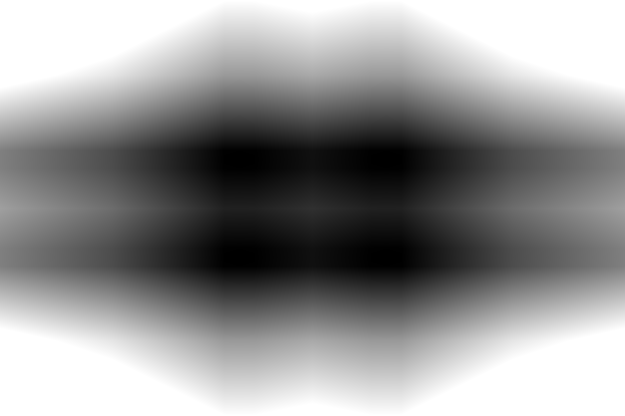
\includegraphics[width=0.8\textwidth]{afsnit/vores_implementation/billeder/udvidet_loesning/topographic_plus.png}}
    \end{center}
    \caption[]{Topografisk kort angivet ved funktionen $t(x, y) =
    \mathbf{X}_x + \mathbf{Y}_y$. Mængden af hvid farve reflekterer
    omkostningen. Helt hvid er dyrest, mens sort er billigst.}
    \label{topography_plus}
\end{figure}

\begin{figure}[h]
    \setlength\fboxsep{0pt}
    \setlength\fboxrule{0.5pt}
    \begin{center}
        \fbox{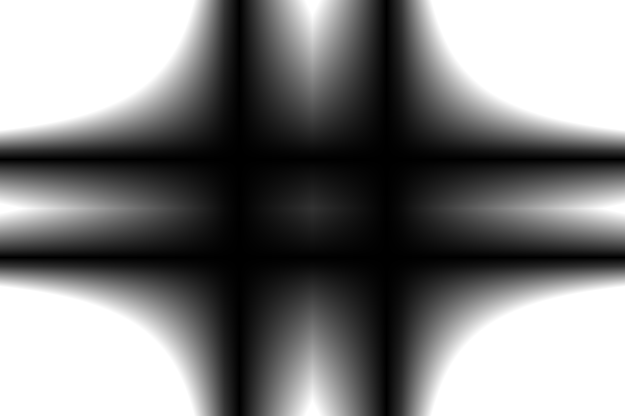
\includegraphics[width=0.8\textwidth]{afsnit/vores_implementation/billeder/udvidet_loesning/topographic_times.png}}
    \end{center}
    \caption[]{Topografisk kort angivet ved funktionen $u(x, y) =
    \mathbf{X}_x\mathbf{Y}_y$. Vi har igen, at hvid farve reflekterer
    omkostningen. Bemærk hvordan det gyldne snit er fremhævet.}
    \label{topography_times}
\end{figure}

\subsubsection*{Fastsættelse af omkostninger}
Det er let at se, at udformningen af det topografiske kort ikke blot
afhænger af funktionen $\tau$, men mere af de værdier man tildeler
omkostningsvektorerne. Værdierne, som er tildelt i det ovenstående, er
valgt arbitrært efter det bedste grafiske resultat. Vi har tidligere
nævnt, at værdierne interpoleres lineært. Hvis man adderer værdierne er
denne metode ikke helt hensigtsmæssig. Det er dog oplagt at gøre brug af
normalfordelingen til at fastsætte omkostninger. Dette skal dog ses med
omvendt fortegn, hvilket betyder, at vi nu tildeler regioner points. Man
kan altså basere antallet af points for et punkt i det et-dimensionelle
plan, ved at bruge en normalfordeling $N(\mu, \sigma)$ med middelværdi
$n\varPhi$ og en passende varians til margin. Umiddelbart ville man
sætte standardafvigelsen til $\delta$, vores margin, hvilket giver os en
varians på $\sigma^{2} = \delta^{2}$. Dette giver os en meget spids
normalfordeling, hvor punkter bliver tildelt mange points for at ligge
inden for margin, men hurtigt aftager når man bevæger sig længere væk.

%\subsubsection*{Fordele og ulemper}
%Brug af omkostninger ved topografiske kort har den umiddelbare fordel at
%kunne tildele regioner en værdi og derved være mere nuanceret i
%bedømmelsen af regioner. Metoden afhænger dog af fornuftige værdier i
%omkostningsvektorerne.

}

% vim: set tw=72 spell spelllang=da:
